\section{First  Implementation and  Discussion}
\label{sec:evaluation}

%% AR
\NEW{In order to play with the new language and do a first evaluation,
a first prototype implementation has been developed on top of 
both  Jason~\cite{jason06}  and  ASTRA~\cite{DBLP:conf/prima/CollierRL15}\footnote{The Jason extension 
is available here: \url{https://github.com/agentspeakers/jason-er}} .

%
The Jason prototype has been used to implement the examples used in this paper.
%
%The new language has been evaluated through a prototype implementation that builds on 
% the ASTRA~\cite{DBLP:conf/prima/CollierRL15} language.  
%
%% AR
The ASTRA prototype uses a syntax slightly different than that used by examples provided in Section~\ref{sec:proposal}, 
being it adapted to the syntactic style adopted in ASTRA.}
%
An example follows:

{\small
\begin{verbatim}
g-plan +!g() : c <: gc { 
  body {
    // main plan body goes here...
    a; b; !g1(); !!g2();
  }

  /* e-plans */
  rule +e1 : c1 { b1; }
  rule +e2 : c2 { b2; }
}
\end{verbatim}}
%
\noindent The different syntax however does not impact the associated semantics.

\NEW{
In the remainder of this section we show the benefits of {\aser} by considering
an existing program, rewritten with the new language.
%
ASTRA is adopted as implementation language---however the same discussion
would apply by considering Jason as implementation language.
}
\subsection{Minority Game}
\label{minority}
% To evaluate our prototype, we have adapted an existing program, introducing {\aser} goal
%rules to a subset of the implementation. Specifically, 

\NEW{We have adapted a simulation of the Minority Game (MG)}, a well-known model for evaluating collective 
behaviour of agents competing  for finite resources~\cite{moro2004minority}. The game involves an odd number of
agents competing for a resource over a series of rounds. For a round, each agent makes a binary
decision (yes/no). At the end of the round, the bids are counted, and the agents that are in the
minority win. The game has been applied mainly in the areas such as modelling financial markets 
\cite{challet2013minority} and traffic simulation \cite{chmura2004minority}.

The existing implementation (see Figure~\ref{fig:mgagents}) consists of 3 types of agent: the 
\emph{compere} agent, who is responsible for managing the game (starting rounds, evaluating bids,
 ...); the \emph{player} agents, who implement a set of MG strategies; and the \emph{main} agent, 
 which is responsible for configuring the game (creating and configuring the compere and player 
 agents). Interaction between the compere and the players is through a shared game-board artifact 
 implemented using CArtAgO~\cite{RicciEPC}.

\begin{figure}[!tbh]
\centering
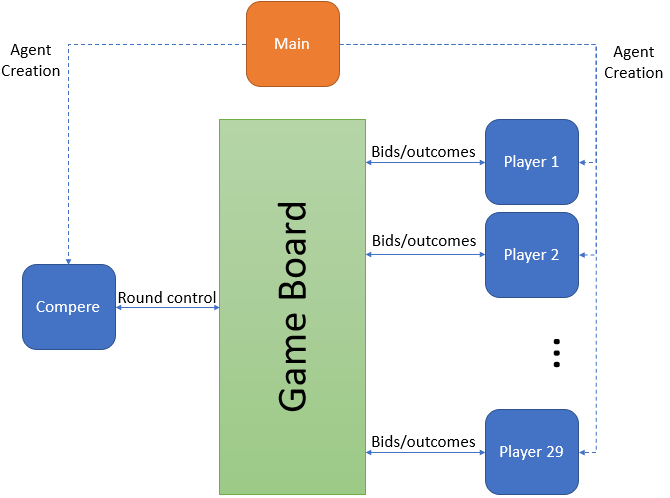
\includegraphics[width=.7\linewidth]{mg.png}
\caption{Minority Game Agent Architecture}
\label{fig:mgagents}
\end{figure}

The existing implementation currently consists of 2 types of plan: \emph{configuration plans}, one of which is
called when the agent is created; and \emph{strategy plans} which implement the various potential strategies
that the agent can use. A subset of the ASTRA implementation of the \emph{player} agent is given below:

{\footnotesize
\begin{verbatim}
  rule +!main(["bestplay", [int t, int h]]) {
    -+strategy("bestplay"); !setup_tactic(t, h); !setup();
  }
  rule +!main([string strategy, []]) { 
    -+strategy(strategy); !setup();
  }
  rule +!setup_tactic(0,int h) {}
  rule +!setup_tactic(int t2, int h) {
    list hist = [];
    int i=0;
    while (i<h) {
      hist = hist + [M.randomInt() % 2];
      i++;
    }
    +strategy(t2, hist, M.randomInt() % 2);
    +score(t2, 0);
    !setup_tactic(t2-1, h);
  }
		
  rule $cartago.signal(string id, play()) : strategy("bestplay") {
    cartago.results(java.util.ArrayList history);
		
    int max_len = -1; int max_choice = -1; int max_score = -1;
    foreach (strategy(int s, list hist, int c) & score(s, int sc)) {
      cartago.match(history, P.fromASTRAList(hist), int len);
      if ((len > max_len) | ((len == max_len) & (max_score < sc))) {
        max_choice = c;	max_score = sc; max_len = len;
      }
    }
    cartago.bid(S.name(), max_choice);
  }
		
  rule $cartago.signal(string id, winner(int bid)) : strategy("bestplay") {
    foreach (strategy(int s, list hist, bid) & score(s, int sc)) {
      -score(s, sc); +score(s, sc+1);
    }
  }
\end{verbatim}}

In the above code, the \verb|!main(...)| plans are the configuration plans. The \verb|!setup_tactic(...)| 
plans are part of the bestplay strategy but are also used for configuration. This is because, unlike
simpler strategies such as \emph{Random Bid} and \emph{Tit-for-Tat}, the best play strategy requires 
that a set of random strategies be created as part of its configuration. In best play, a random strategy is
a randomly generated set of \verb|h| outcomes combined with a recommended next move. Each strategy has 
an associated score which is used to help determine how successful each strategy is.

The strategy plans are the \verb|$cartago.signal(...)| plans, which handle the \verb|play()| 
and \verb|winner(...)| signals respectively. These signals are generated by the game board when 
the  \emph{compere} agent performs operations on it (e.g. when a round starts/ends). For bestplay, the 
\verb|play()| signal triggers a behaviour where the agent compares the game outcome history against 
its strategies and picks the strategy that best fits the history (longest matching subsequence). The
corresponding next move is played (via the \verb|bid()| artifact operation). Conversely, the 
\verb|winner(...)| signal triggers a behaviour where the agent updating the score for all 
strategies that lead to \verb|bid| being selected.

Some of the key points to note when reviewing the above code are: (i) a custom plan is needed 
to handle the \verb|!main(...)| goal in the case of the bestplay strategy because it requires
some custom initialisation; (ii) a strategy belief is required to enable the identification of the
plans that are relevant to the selected strategy; and (iii) there is no guarantee that these
plans will be grouped together in the implemented agent. They could be spread throughout the
agents codebase making it difficult to read and understand the overall behaviour.

In the {\aser} implementation, we still maintain the two types of plan, however instead on needing
multiple plans to capture a strategy, the entire strategy is now encapsulated within a single
g-plan (of course the other plans still exist as subplans of the g-plan). The snippet of code 
below contains the {\aser} code to the ASTRA example given above:

{\footnotesize
\begin{verbatim}
  rule +!main([string strategy, list config]) {
    !win(strategy, config);
  }
  
  g-rule +!win("bestplay", [int t, int h]) { % <: false {
    body {
      !setup_tactic(t);
    }

    rule +!setup_tactic(0) {}
    rule +!setup_tactic(int t2) {
      list hist = [];
      int i=0;
      while (i<h) {
        hist = hist + [M.randomInt() % 2];
        i++;
      }
      +strategy(t2, hist, M.randomInt() % 2);
      +score(t2, 0);
      !setup_tactic(t2-1);
    }

    rule $cartago.signal(string id, play()) {
      cartago.results(java.util.ArrayList history);
			
      int max_len = -1; int max_choice = -1; int max_score = -1;
      foreach (strategy(int s, list hist, int c) & score(s, int sc)) {
        cartago.match(history, P.fromASTRAList(hist), int len);
        if ((len > max_len) | ((len == max_len) & (max_score < sc))) {
          max_choice = c; max_score = sc; max_len = len;
        }
      }		
      cartago.bid(S.name(), max_choice);
    }
		
    rule $cartago.signal(string id, winner(int bid)) {
      foreach (strategy(int s, list hist, bid) & score(s, int sc)) {
        -score(s, sc); +score(s, sc+1);
      }
    }
  }
\end{verbatim}}

As can be seen from the above snippet of code. The implementation of the two types of agent
is quite similar. In fact many of the rule implementations have not changed significantly.
However, there are a few interesting observations regarding the revised implementation: \emph{(i)} the 
complexity of the plan contexts were simplified when using g-plans because the g-plan itself 
provided some of the context; \emph{(ii)} the number of arguments passed as parameters was reduced, 
again because the scope of the parameters of the g-plan was the plan body \emph{and} all of 
its sub-plans; \emph{(iii)} the total number of rules under consideration on each iteration was
significantly less because only the rules within an active g-plan were considered by the
agent. This means that, when an agent has multiple strategies, only the rules relating to
the active strategy will be considered, whereas in ASTRA, all rules are always considered.

\subsection{A Note on Performance}
\label{performance}

After reviewing our new language, it became apparent that (i) it was reducing the number of plans 
that need to be evaluated on each iteration; but (ii) the introduction of a goal condition introduces
a significant new overhead because it must be evaluated on each iteration.
As a result, it was decided that a comparison of the new and old languages be carried out. Initially,
we compared interpreter cycle execution time and the number of iterations based on a single 
configuration of the MG with 29 players and 1000 rounds. For our results, we averaged
the values across all 29 players and repeated the experiment 5 times.

\begin{table}[]
\centering
\caption{Comparing ASTRA and {\aser}}
\label{comparison}
\begin{tabular}{lrrrr}
                            & ASER    & ASTRA  \\ \toprule
Cycle Time (ms)             & 0.0017  & 0.0036 \\
Cycles                      & 293,772 & 62,880 \\
Elapsed Execution Time (ms) & 495.22  & 229.29 \\
Unix (timed)                & 16s     & 15s   
\end{tabular}
\end{table}

Results of our initial comparison can be found in Table~\ref{comparison}. The difference
in the number of cycles is due primarily to the scheduling algorithm used by ASTRA, which
suspends agents that have no sensors (perceptors) and whose event and intention queues are empty.
The impact of this is that ASTRA is generally more efficient than {\aser}. Due to the small but 
consistent difference in performance between the unix timing of the two experiments, we then 
explored how increasing the number of rounds affected performance. Results for this are shown 
in Table~\ref{rounds}.

\begin{table}[]
\centering
\caption{ASTRA vs {\aser} Performance}
\label{rounds}
\begin{tabular}{lrrrrr}
           & 1000   & 2000   & 3000   & 4000   & 10000   \\ \toprule
ASER (s)   & 15.514 & 30.251 & 44.202 & 57.736 & 140.059 \\
ASTRA (s)  & 14.893 & 28.232 & 42.168 & 56.453 & 137.379 \\
Diff. (\%) & 4.2\%  & 6.8\%  & 4.8\%  & 2.3\%  & 2.0\%  
\end{tabular}
\end{table}

This second table shows that the introduction of g-rules in {\aser} has only a small impact on 
performance. Here, it is almost linear. Further, ASTRA shows a marginal performance improvement of between 2-6\%.

While this is not intended to be a thorough evaluation of {\aser}, it is useful because
it hints that the use of goal conditions does not significantly impact the performance 
of the language. It must also be noted that the prototype implementation is not as mature 
as the ASTRA implementation --- interpreter optimisations could further reduce the difference 
in performance.
